% !TeX root = surprises.tex

\selectlanguage{hebrew}


\chapter{משפט חמשת הצבעים}
\label{c.five}


\section{מפות מישוריות וגרפים מישוריים}\label{s.planar}

\begin{theorem}\mbox{}\\
ניתן לצבוע מפה מישורית עם ארבעה צבעים כך ששני שטחים שכנים צבועים בצבע שונה.
\end{theorem}

הוכחת משפט זה קשה ביותר; כאן נוכיח משפט הרבה יותר קל, משפט חמשת הצבעים שהוכח במאה התשע-עשרה.

\begin{theorem}\mbox{}\\
ניתן לצבוע מפה מישורית עם חמישה צבעים כך ששני שטחים שכנים צבועים בצבעים שונים.
\end{theorem}

\textbf{הגדרה:}
\textbf{מפה מישורית}
היא אוסף של שטחים במישור עם גבולות משותפים.
\textbf{צביעה}
של מפה היא השמה של צבעים לשטחים כך שכל זוג שטחים שיש להם גבולות  משותפים צבועים בצבעים שונים.%
\footnote{%
שטחים שאין להם גבול משותף יכולים להיחשב כשייכים "לאותה ארץ", למשל, אלסקה היא חלק מארה"ב. בבעיה המתימטית, נתייחס אליהם  כשטחים שונים שניתן לצבוע באותו צבע או בצבעים שונים.%
}

האיור שלהלן
%\ref{f.maps}
מראה שתי בצביעות שונות למפה מישורית עם עשרה שטחים: משמאל חמישה צבעים ומימין עם ארבעה צבעים.
%\begin{figure}{bt}
\begin{center}

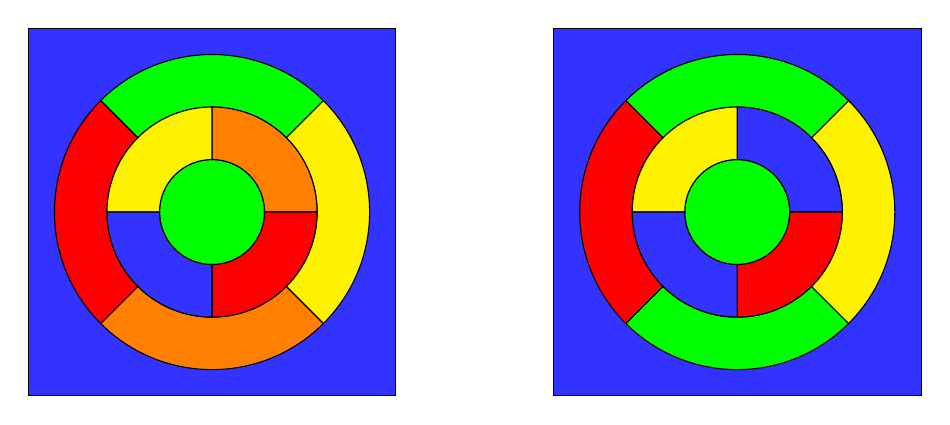
\begin{tikzpicture}[scale=.667]
\draw[fill=blue!80] (-3.5,-3.5) rectangle +(7,7);

\draw[fill=green] (0:1) 
  arc [start angle=0,  end angle=360, radius=1];

\draw[fill=green] (45:2) --
      (45:3)  arc[start angle=45,  end angle=135, radius=3] --
      (135:2) arc[start angle=135, end angle=45,  radius=2];
\draw[fill=orange] (-45:2) --
      (-45:3)  arc[start angle=-45,  end angle=-135, radius=3] --
      (-135:2) arc[start angle=-135, end angle=-45,  radius=2];
\draw[fill=yellow] (45:2) --
      (45:3)  arc[start angle=45,  end angle=-45, radius=3] --
      (-45:2) arc[start angle=-45, end angle=45,  radius=2];
\draw[fill=red] (135:2) --
      (135:3)  arc[start angle=135,  end angle=225, radius=3] --
      (225:2) arc[start angle=225, end angle=135,  radius=2];

\draw[fill=orange] (0:1) --
      (0:2)  arc[start angle=0,  end angle=90, radius=2] --
      (90:1) arc[start angle=90, end angle=0,  radius=1];
\draw[fill=red] (0:1) --
      (0:2)  arc[start angle=0,  end angle=-90, radius=2] --
      (-90:1) arc[start angle=-90, end angle=0,  radius=1];
\draw[fill=yellow] (90:1) --
      (90:2)  arc[start angle=90,  end angle=180, radius=2] --
      (180:1) arc[start angle=180, end angle=90,  radius=1];
\draw[fill=blue!80] (180:1) --
      (180:2)  arc[start angle=180,  end angle=270, radius=2] --
      (270:1) arc[start angle=270, end angle=180,  radius=1];

\begin{scope}[xshift=10cm]
\draw[fill=blue!80] (-3.5,-3.5) rectangle +(7,7);

\draw[fill=green] (0:1) 
  arc [start angle=0,  end angle=360, radius=1];

\draw[fill=green] (45:2) --
      (45:3)  arc[start angle=45,  end angle=135, radius=3] --
      (135:2) arc[start angle=135, end angle=45,  radius=2];
\draw[fill=green] (-45:2) --
      (-45:3)  arc[start angle=-45,  end angle=-135, radius=3] --
      (-135:2) arc[start angle=-135, end angle=-45,  radius=2];
\draw[fill=yellow] (45:2) --
      (45:3)  arc[start angle=45,  end angle=-45, radius=3] --
      (-45:2) arc[start angle=-45, end angle=45,  radius=2];
\draw[fill=red] (135:2) --
      (135:3)  arc[start angle=135,  end angle=225, radius=3] --
      (225:2) arc[start angle=225, end angle=135,  radius=2];

\draw[fill=blue!80] (0:1) --
      (0:2)  arc[start angle=0,  end angle=90, radius=2] --
      (90:1) arc[start angle=90, end angle=0,  radius=1];
\draw[fill=red] (0:1) --
      (0:2)  arc[start angle=0,  end angle=-90, radius=2] --
      (-90:1) arc[start angle=-90, end angle=0,  radius=1];
\draw[fill=yellow] (90:1) --
      (90:2)  arc[start angle=90,  end angle=180, radius=2] --
      (180:1) arc[start angle=180, end angle=90,  radius=1];
\draw[fill=blue!80] (180:1) --
      (180:2)  arc[start angle=180,  end angle=270, radius=2] --
      (270:1) arc[start angle=270, end angle=180,  radius=1];
\end{scope}
\end{tikzpicture}
\end{center}
%\caption{צביעת מפות}\label{f.maps}
%\end{figure}

\textbf{הגדרה:}
\textbf{גרף}
הוא קבוצה של 
\textbf{צמתים}
$V$
וקבוצה של 
\textbf{קשתות}
$E$,
כך שכל קשת מחבר בדיוק שני צמתים.
\textbf{גרף מישורי}
הוא גרף בו שתי קשתות לא חותכות אחת את השניה. בגרף מישורי קטע מהמישור התחום על ידי קבוצה של קשתות נקרא 
\textbf{שטח}.
\textbf{צביעה}
של גרף מישורי היא השמה של צבעים לצמתים כך ששני צמתים המחוברים על ידי קשת צבועים בצבעים שונים.

%

מפות וגרפים דואליים ונוח יותר לטפל בבעיות צביעה בגרפים ולא במפות.
\begin{theorem}\mbox{}\\
נתונה מפה מישורית, ניתן לבנות גרף מישורי כך שעבור כל צביעה של שטחים במפה קיימת צביעה של הצמתים בגרף, ולהיפך.
\end{theorem}

\textbf{הוכחה:}
בנו צומת עבור כל שטח במפה ובנו קשת בין שני צמתים אם ורק אם קיים גבול בין שני השטחים.
\qed

האיור שלהן
%\ref{f.map-graph}
מראה את הגרף המישורי שניתן לבנות מהמפה המישורית שהבאנו לעיל:
%\begin{figure}[tb]
\begin{center}

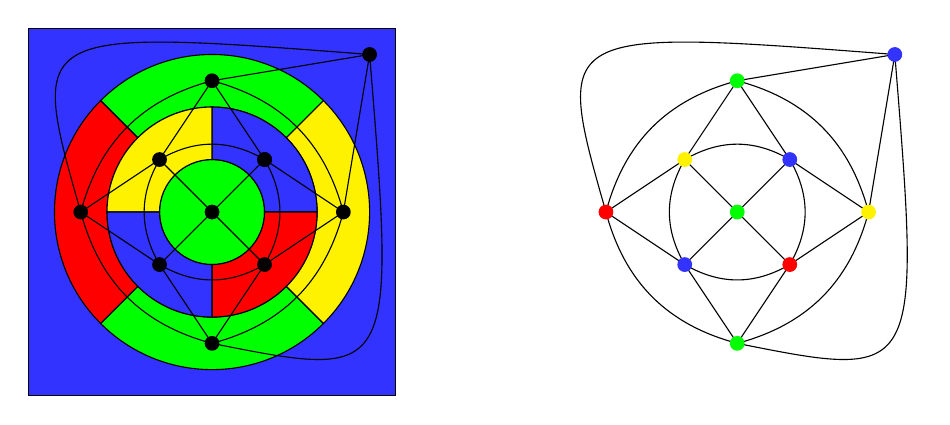
\begin{tikzpicture}[scale=.667]

\draw[fill=blue!80] (-3.5,-3.5) rectangle +(7,7);

\draw[fill=green] (0:1) 
  arc [start angle=0,  end angle=360, radius=1];

\draw[fill=green] (45:2) --
      (45:3)  arc[start angle=45,  end angle=135, radius=3] --
      (135:2) arc[start angle=135, end angle=45,  radius=2];
\draw[fill=green] (-45:2) --
      (-45:3)  arc[start angle=-45,  end angle=-135, radius=3] --
      (-135:2) arc[start angle=-135, end angle=-45,  radius=2];
\draw[fill=yellow] (45:2) --
      (45:3)  arc[start angle=45,  end angle=-45, radius=3] --
      (-45:2) arc[start angle=-45, end angle=45,  radius=2];
\draw[fill=red] (135:2) --
      (135:3)  arc[start angle=135,  end angle=225, radius=3] --
      (225:2) arc[start angle=225, end angle=135,  radius=2];

\draw[fill=blue!80] (0:1) --
      (0:2)  arc[start angle=0,  end angle=90, radius=2] --
      (90:1) arc[start angle=90, end angle=0,  radius=1];
\draw[fill=red] (0:1) --
      (0:2)  arc[start angle=0,  end angle=-90, radius=2] --
      (-90:1) arc[start angle=-90, end angle=0,  radius=1];
\draw[fill=yellow] (90:1) --
      (90:2)  arc[start angle=90,  end angle=180, radius=2] --
      (180:1) arc[start angle=180, end angle=90,  radius=1];
\draw[fill=blue!80] (180:1) --
      (180:2)  arc[start angle=180,  end angle=270, radius=2] --
      (270:1) arc[start angle=270, end angle=180,  radius=1];


\foreach \x/\y/\name in {
    0/0/O,
    3/3/Z,
    1/1/E,-1/1/F,-1/-1/G,1/-1/H,
    0/2.5/A,2.5/0/B,0/-2.5/C,-2.5/0/D,
    } {
  \fill (\x,\y) coordinate(\name) circle(4pt);
}

\draw (E) -- (O) -- (F);
\draw (G) -- (O) -- (H);
\draw (E) to [bend right=30] (F) to [bend right=30] (G) 
          to [bend right=30] (H) to [bend right=30] (E);
\draw (A) -- (E) -- (B) -- (H) -- (C) -- (G) -- (D) -- (F);
\draw (A) to [bend right=30] (D) to [bend right=30] (C) 
          to [bend right=30] (B) to [bend right=30] (A);

\draw (F) -- (A) -- (Z) -- (B);
\draw (C) .. controls (3.5,-3.2) .. (Z);
\draw (D) .. controls (-3.5,3.5) .. (Z);

\begin{scope}[xshift=10cm]

\foreach \x/\y/\name in {
    0/0/O,
    3/3/Z,
    1/1/E,-1/1/F,-1/-1/G,1/-1/H,
    0/2.5/A,2.5/0/B,0/-2.5/C,-2.5/0/D,
    } {
  \coordinate(\name) at (\x,\y);
}

\draw (E) -- (O) -- (F);
\draw (G) -- (O) -- (H);
\draw (E) to [bend right=30] (F) to [bend right=30] (G) 
          to [bend right=30] (H) to [bend right=30] (E);
\draw (A) -- (E) -- (B) -- (H) -- (C) -- (G) -- (D) -- (F);
\draw (A) to [bend right=30] (D) to [bend right=30] (C) 
          to [bend right=30] (B) to [bend right=30] (A);

\draw (F) -- (A) -- (Z) -- (B);
\draw (C) .. controls (3.5,-3.2) .. (Z);
\draw (D) .. controls (-3.5,3.5) .. (Z);

\foreach \cl/\x/\y in {
    green/0cm/0cm,
    blue!80/3cm/3cm,
    blue!80/1cm/1cm,
    yellow/-1cm/1cm,
    blue!80/-1cm/-1cm,
    red/1cm/-1cm,
    green/0cm/2.5cm,
    yellow/2.5cm/0cm,
    green/0cm/-2.5cm,
    red/-2.5cm/0cm
    }
  \fill[\cl] (\x,\y) circle (4pt);
\end{scope}
\end{tikzpicture}
\end{center}
%\caption{גרף שקול למפה}\label{f.map-graph}
%\end{figure}
ניתן להגביל את עצמנו לגרפים שהשטחים שלהם
\textbf{משולשיים}.%
\footnote{%
השטחים הם לא בהכרח 
\textbf{משולשים}
כי הקשתות יכולות להיות עקומות. לפי משפט
\L{F\'{a}ry},
כל גרף מישורי משולשי ניתן להפוך לגרף מישורי שקול עם קשתות ישרות.%
}

האיור השמאלי שלהלן מראה צביעת ריבוע עם שני צבעים, אבל אם 
\textbf{מתלתים}
\L{(triangulate)} 
אותו )איור מרכזי(, חייבים להשתמש בארבעה צבעים. היעד הוא להוכיח 
\textbf{שכל}
גרף ניתן לצבוע בחמישה צבעים, כך שאם הדבר אפשרי בגרף המשולשי, הוא אפשרי גם בגרף המקורי, כי מחיקת הקשתות הנוספות לא מקלקלת את הצביעה )איור ימני(.
\begin{center}

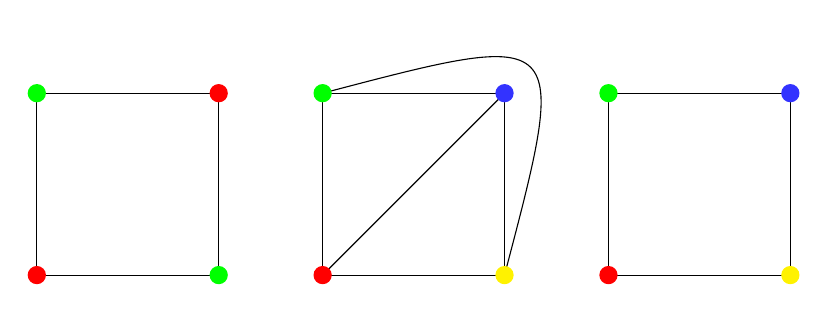
\begin{tikzpicture}[scale=.33]
\draw (-3.5,-3.5) rectangle +(7,7);
\fill[red] (-3.5,-3.5) circle(10pt);
\fill[green] (-3.5,3.5) circle(10pt);
\fill[green] (3.5,-3.5) circle(10pt);
\fill[red] (3.5,3.5) circle(10pt);
\begin{scope}[xshift=11cm]
\draw (-3.5,-3.5) -- (3.5,3.5);
\draw (-3.5,3.5) .. controls (6,6) .. (3.5,-3.5);
\draw (-3.5,-3.5) rectangle +(7,7);
\fill[red] (-3.5,-3.5) circle(10pt);
\fill[green] (-3.5,3.5) circle(10pt);
\fill[yellow] (3.5,-3.5) circle(10pt);
\fill[blue!80] (3.5,3.5) circle(10pt);
\end{scope}
\begin{scope}[xshift=22cm]
\draw (-3.5,-3.5) rectangle +(7,7);
\fill[red] (-3.5,-3.5) circle(10pt);
\fill[green] (-3.5,3.5) circle(10pt);
\fill[yellow] (3.5,-3.5) circle(10pt);
\fill[blue!80] (3.5,3.5) circle(10pt);
\end{scope}
\end{tikzpicture}
\end{center}

\selectlanguage{hebrew}


\section{הנוסחה של
\L{Euler}}

\begin{theorem}[\L{Euler}]\label{thm.euler}\mbox{}\\
יהי
$G$
גרף מישורי מקושר עם
$V$
צמתים,
$E$
קשתות ו-%
$F$
שטחים. אזי
$V-E+F=2$.
\end{theorem}

\textbf{הוכחה:}
באינדוקציה על מספר הקשתות. אם מספר הקשתות בגרף מישורי מקושר הוא אפס, קיים רק צומת אחד ושטח אחד כך ש-%
$1-0+1=2$.

יהי 
$G$
גרף מישורי מקושר עם 
$V$
צמתים, 
$E$
קשתות ו-%
$F$
שטחים, ומחק קשת 
$e$
המחבר את הצמתים
$v_1,v_2$.


\textbf{מקרה 1:}
הגרף מפסיק להיות מקושר )איור שמאלי(. זהה את
$v_1$
עם
$v_2$
)איור ימני(.
ל-%
$G'$,
הגרף הנוצר, פחות קשתות מ-%
$G$,
הוא גרף מישורי מקושר,
ולכן לפי הנחת האינדוקציה,
$(V-1)-(E-1)+F=2$
כי יש גם צומת אחד פחות. נפשט ונקבל
$V-E+F=2$
עבור
$G$.

\begin{center}

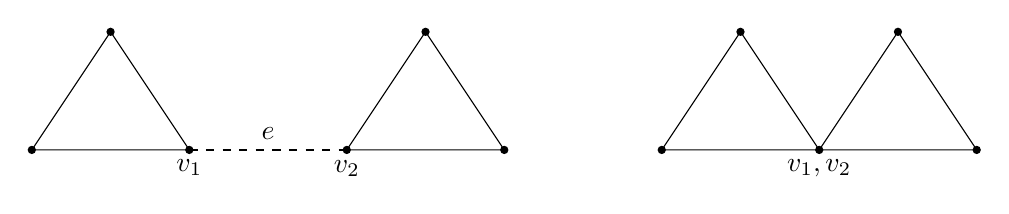
\begin{tikzpicture}
\foreach \x/\y in {0/0, 2/0, 1/1.5,4/0,6/0,5/1.5}
  \fill (\x,\y) circle (1.5pt);
\draw (2,0) -- (1,1.5) -- (0,0) -- (2,0) node[below] {$v_1$};
\draw[dashed,thick] (2,0) -- node[above] {$e$} (4,0) node[below] {$v_2$};
\draw (4,0) -- (6,0) -- (5,1.5) -- (4,0);
\begin{scope}[xshift=8cm]
\foreach \x/\y in {0/0, 2/0, 1/1.5,4/0,3/1.5}
  \fill (\x,\y) circle (1.5pt);
\draw (2,0) -- (1,1.5) -- (0,0) -- (2,0) node[below] {$v_1,v_2$} -- (4,0) -- (3,1.5) -- (2,0);
\end{scope}
\end{tikzpicture}
\end{center}

\textbf{מקרה 2:}
הגרף נשאר מקושר. לגרף הנוצר
$G'$
פחות קשתות מ-%
$G$,
ולכן לפי הנחת האינדוקציה,
$V-(E-1)+(F-1)=2$
כי מחיקת קשת אחת מאחדת שני שטחים לאחד. נפשט ונקבל
$V-E+F=2$ 
עבור
$G$.
\qed

\begin{center}

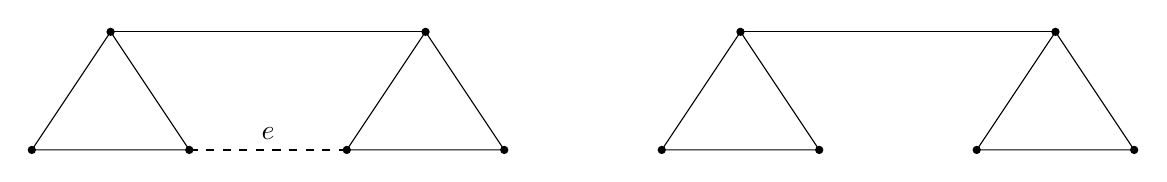
\begin{tikzpicture}
\foreach \x/\y in {0/0, 2/0, 1/1.5,4/0,6/0,5/1.5}
  \fill (\x,\y) circle (1.5pt);
\draw (2,0) -- (1,1.5) -- (0,0) -- (2,0);
\draw[thick,dashed] (2,0) -- node[above] {$e$} (4,0);
\draw (4,0) -- (6,0) -- (5,1.5) -- (4,0);
\draw (1,1.5) -- (5,1.5);
\begin{scope}[xshift=8cm]
\foreach \x/\y in {0/0, 2/0, 1/1.5,4/0,6/0,5/1.5}
  \fill (\x,\y) circle (1.5pt);
\draw (2,0) -- (1,1.5) -- (0,0) -- (2,0);
\draw (4,0) -- (5,1.5) -- (6,0) -- cycle;
\draw (1,1.5) -- (5,1.5);
\end{scope}
\end{tikzpicture}
\end{center}
\begin{theorem}\mbox{}\\
יהי
$G$
גרף מישורי מקושר ומתולת. אזי
$E= 3V-6$.
\end{theorem}
למשל, בגרף המישורי בסעיף
\L{~\ref{s.planar}}
יש
$10$
צמתים ו-%
$24= 3\cdot 10-6$
קשתות.

\textbf{הוכחה:}
כל שטח חסום על ידי שלוש קשתות, כך ש-%
$E=3F/2$
כי כל קשת נספר פעמיים, פעם אחת לכל שטח שהיא חוסמת. לפי נוסחת
\L{Euler}:

\begin{eqn}
E&=&V+F-2\\
E&=&V+2E/3-2\\
E&=&3V-6\,.
\end{eqn}\qed

\begin{theorem}\label{thm.count}\mbox{}\\
יהי
$G$
גרף מישורי מקושר. אזי
$E\leq 3V-6$.
\end{theorem}
עבור הגרף באיור שלהלן,
$E=8\leq 3\cdot 6 - 6= 12$.

\begin{center}

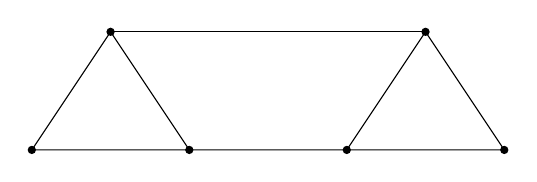
\begin{tikzpicture}
\foreach \x/\y in {0/0, 2/0, 1/1.5,4/0,6/0,5/1.5}
  \fill (\x,\y) circle (1.5pt);
\draw (2,0) -- (1,1.5) -- (0,0) -- (2,0) -- (4,0) -- (6,0) -- (5,1.5) -- (4,0);
\draw (1,1.5) -- (5,1.5);
\end{tikzpicture}
\end{center}

\textbf{הוכחה:}
תלתו את
$G$
כדי לקבל
$G'$.
ב-%
$G'$, $E= 3V-6$
לפי משפט~%
\L{\ref{thm.count}}.
כעת, מחק קשתות מ-%
$G'$
כדי לקבל את
$G$.
מספר הצמתים לא משתנה כך ש-%
$E\leq 3V-6$.\qed

הנה הגרף המתולת שעבורו
$E=3\cdot 6 - 6= 12$.
\begin{center}

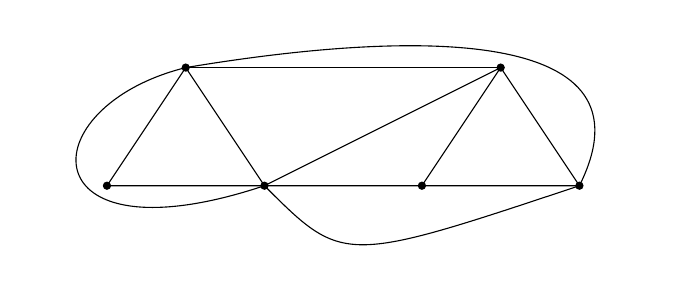
\begin{tikzpicture}
\foreach \x/\y in {0/0, 2/0, 1/1.5,4/0,6/0,5/1.5}
  \fill (\x,\y) circle (1.5pt);
\draw (2,0) -- (1,1.5) -- (0,0) -- (2,0) -- (4,0) -- (6,0) -- (5,1.5) -- (4,0);
\draw (1,1.5) -- (5,1.5);
\draw (2,0) -- (5,1.5);
\draw (2,0) .. controls (-1,-1) and (-1,1) .. (1,1.5);
\draw (2,0) .. controls (3,-1) .. (6,0) .. controls (7,2) and (4,2) .. (1,1.5);
\end{tikzpicture}
\end{center}

\selectlanguage{hebrew}


\section{גרפים שאינם מישוריים}
נסטה מעט מהסיפור כדי להראות איך ניתן להשתמש במשפטים 
\L{~\ref{thm.euler}}
ו-%
\L{~\ref{thm.count}}
כדי להוכיח שגרפים מסויימים אינם מישוריים.

\begin{theorem}\mbox{}\\
$K_5$,
הגרף השלם עם חמישה צמתים אינו מישורי.
\end{theorem}
%\begin{figure}[bt]
\begin{center}

\begin{tikzpicture}[scale=.8]
\node (pentagon) [minimum size=4cm,regular polygon,regular polygon sides=5] at (0,0) {};
\draw (pentagon.corner 1) -- (pentagon.corner 2);
\draw (pentagon.corner 2) -- (pentagon.corner 3);
\draw (pentagon.corner 3) -- (pentagon.corner 4);
\draw (pentagon.corner 4) -- (pentagon.corner 5);
\draw (pentagon.corner 5) -- (pentagon.corner 1);
\draw (pentagon.corner 1) -- (pentagon.corner 3);
\draw (pentagon.corner 1) -- (pentagon.corner 4);
\draw (pentagon.corner 2) -- (pentagon.corner 4);
\draw (pentagon.corner 2) -- (pentagon.corner 5);
\draw (pentagon.corner 3) -- (pentagon.corner 5);

\foreach \corner in {1,2,3,4,5}
  \fill (pentagon.corner \corner) circle (2pt);

\begin{scope}[xshift=8cm]
\node (pentagon) [minimum size=4cm,regular polygon,regular polygon sides=5] at (0,0) {};
\draw (pentagon.corner 1) -- (pentagon.corner 2);
\draw (pentagon.corner 2) -- (pentagon.corner 3);
\draw (pentagon.corner 3) -- (pentagon.corner 4);
\draw (pentagon.corner 4) -- (pentagon.corner 5);
\draw (pentagon.corner 5) -- (pentagon.corner 1);
\draw (pentagon.corner 1) .. controls (-4,1) .. 
      (pentagon.corner 3);
\draw (pentagon.corner 1) .. controls (4,1) ..
      (pentagon.corner 4);
\draw (pentagon.corner 2) -- (pentagon.corner 4);
\draw (pentagon.corner 2) -- (pentagon.corner 5);
\draw (pentagon.corner 3) -- (pentagon.corner 5);

\foreach \corner in {1,2,3,4,5}
  \fill (pentagon.corner \corner) circle (2pt);
\draw (0,-.95) circle(5pt);
\end{scope}
\end{tikzpicture}
\end{center}
%\caption{גרף שלם על עם חמישה קודקודים}\label{f.k5}
%\end{figure}
\textbf{הוכחה:}
עבור
$K_5$, $V=5$
ו-%
$E=10$.
אבל
$10 \not\leq 3\cdot 5 -6=9$.\qed

\begin{theorem}\mbox{}\\
$K_{3,3}$,
הגרף הדו-אזורי עם שלושה צמתים בכל איזור )איור שמאלי(,
אינו מישורי.
\end{theorem}
%\begin{figure}[tb]
\begin{center}

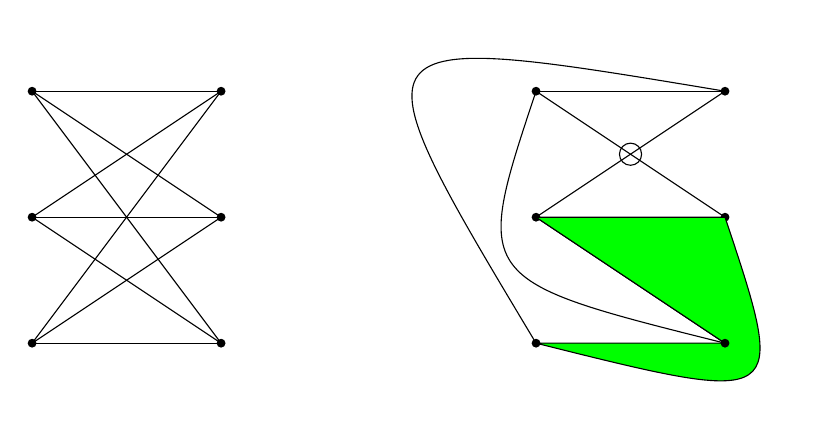
\begin{tikzpicture}[scale=.8]
\foreach \x/\y in {0/0,0/2,0/4,3/0,3/2,3/4}
  \fill (\x,\y) circle (2pt);
\draw (0,0) -- (3,0);
\draw (0,2) -- (3,2);
\draw (0,4) -- (3,4);
\draw (0,0) -- (3,2);
\draw (0,2) -- (3,4);
\draw (0,4) -- (3,0);
\draw (0,0) -- (3,4);
\draw (0,2) -- (3,0);
\draw (0,4) -- (3,2);
\begin{scope}[xshift=8cm]
\foreach \x/\y in {0/0,0/2,0/4,3/0,3/2,3/4}
  \fill (\x,\y) circle (2pt);
\draw (0,4) -- (3,4);
c\draw (0,2) -- (3,4);
\draw (0,4) .. controls (-1,1) .. (3,0);
\draw (0,0) .. controls (-3,5) .. (3,4);
\draw (0,2) -- (3,0);
\draw (0,4) -- (3,2);

\draw[fill=green] (0,0) -- (3,0) -- (3,0) -- (0,2)  -- (3,2) .. controls (4,-1) .. (0,0);
\fill (3,0) circle (2pt);
\draw (1.5,3) circle(5pt);
\end{scope}
\end{tikzpicture}
\end{center}
%\caption{גרף דו-איזורי עם שלושה צמתים בכל איזור}\label{f.k33}
%\end{figure}
\textbf{הוכחה:}
$V=6$
ו-%
$E=9$.
לפי משפט
\L{~\ref{thm.euler}},
$F=E-V+2=9-6+2=5$.
אבל כל שטח תחום על ידי ארבע קשתות )איור ימני(, ולכן
$E=4F/2=(4\cdot 5)/2\neq 9$.\qed


\selectlanguage{hebrew}


\section{המעלה של הצמתים}

\begin{definition}
$d(v)$,
\textbf{המעלה}
של צומת
$v$,
היא מספר הקשתות הנפגשות ב-%
$v$.
\end{definition}

עבור הגרף בסעיף
\L{~\ref{s.planar}},
קיימים 
$8$
צמתים בתוך הטבעות, כל אחד ממעלה
$5$.
המעלה של השטח החיצוני ושל המעגל הפנימי הוא 
$4$.
לכן:
\[
\sum_{v\in V} d(v) = 5\cdot 8 + 4\cdot 2=48\,.
\]
נקבל את מספר הקשתות בגרף על ידי חלוקת סכום המעלות ב-%
$2$,
כי כל קשת נספרה פעמיים, פעם אחת עבור כל צומת שהיא נוגעת בו.
הכללת הטיעונים הללו מוכיחה:
\begin{theorem}\label{thm.degrees}\mbox{}\\
יהי
$d_i, i=1,2,3,\ldots,k$
מספרי הצמתים ממעלה
$i$
בגרף מישורי מקושר עם
$V$
צמתים ו-%
$E$ 
קשתות, כאשר
$k$
הוא המעלה הגבוהה ביותר של צומת ב-%
$V$.
אזי:
\[
\sum_{v\in V} d(v) =\sum_{i=1}^{k} i\cdot d_i=2E\,.
\]
\end{theorem}
\vspace*{-6ex}
\begin{theorem}\label{thm.degree5}\mbox{}\\
יהי
$G$
גרף מישורי מקושר עם
$E$
קשתות ו-%
$V$
צמתים, ויהי
$d_i,i=1,\ldots,k$
מספרי ההצמתים ממעלה
$i$,
כאשר
$k$
הוא המעלה הגבוהה ביותר של צומת ב-%
$V$.
אזי חייב להיות צומת
$v$
ב-%
$V$
כך ש-%
$d(v) \leq 5$.
\end{theorem}
\textbf{הוכחה 1:}
ברור שאם יש 
$d_1$
צמתים ממעלה
$1$, $d_2$ 
צמתים ממעלה
$2$, \ldots, $d_k$
צמתים ממעלה
$k$, 
אזי
$V=\sum_{i=1}^{k}d_i$. 
מהמשפטים
\L{~\ref{thm.count}}
ו-%
\L{~\ref{thm.degrees}}
נקבל:
\[
\sum_{i=1}^{k} i\cdot d_i=2E\leq 2(3V-6) = 6V-12=6\sum_{i=1}^{k} d_i -12\,.
\]
מכאן ש:
\[
\sum_{i=1}^{k} i\cdot d_i \leq 6\sum_{i=1}^{k} d_i -12\,,
\]
ו:
\[
\sum_{i=1}^{k} (6-i)d_i\geq 12\,.
\]
בגלל ש-%
$12>0$,
ל-%
$i$
אחד לפחות,
$6-i>0$
ועבור 
$i$
זה,
$i<6$. 
\qed

\textbf{הוכחה 2:}
נחשב את 
\textbf{הממוצע}
של המעלות של הצמתים שהוא סכום המעלות לחלק למספר הצמתים:
\[
d_{\textit{\footnotesize avg}}=\frac{\sum_{i=1}^{k} i\cdot d_i}{V}\,.
\]
אבל סכום המעלות הוא פעמיים מספר הקשתות, ולפי משפט
\L{~\ref{thm.count}}
נקבל:
\[
d_{\textit{\footnotesize avg}}=\frac{2E}{V}\leq \frac{6V-12}{V}=6-\frac{6}{V}<6\,.
\]
אם 
\textbf{הממוצע}
של המעלות הוא פחות משש, חייב להיות צומת אחד לפחות ממעלה פחות משש.
\qed


עבור הגרף בסעיף
\L{~\ref{s.planar}},
סכום המעלות הוא
$8\cdot 5 + 2\cdot 4=48$.
יש 
$10$
צמתים, כך שממוצע המעלות שלו הוא
$\frac{48}{10}=4.8$
וחייב להיות צומת ממעלה 
$4$
או פחות.

\selectlanguage{hebrew}



\section{משפט ששת הבצעים}

\begin{theorem}\label{thm.sixcolor}\mbox{}\\
כל גרף מישורי ניתן לצביעה בששה צבעים.
\end{theorem}
\textbf{הוכחה:}
באינדוקציה על מספר הצמתים ב-%
$G$.
אם לגרף ששה צמתים או פחות, ברור שניתן לצבוע את הגרף בששה צבעים.

יהי
$G$
גרף מישורי. לפי משפט
\L{~\ref{thm.degree5}}
קיים צומת
$v$
ממעלה חמש או פחות. מחק צומת
$v$
כדי לקבל את הגרף
$G'$.
לפי הנחת האינדוקציה, ניתן לצבוע את
$G'$
עם ששה צבעים, אבל ל-%
$v$
חמישה שכנים לכל היותר שצבועים בחמישה 
צבעים לכל היותר, כך שנשאר צבע ששי שניתן לצבוע בו את
$v$. \qed

\begin{center}

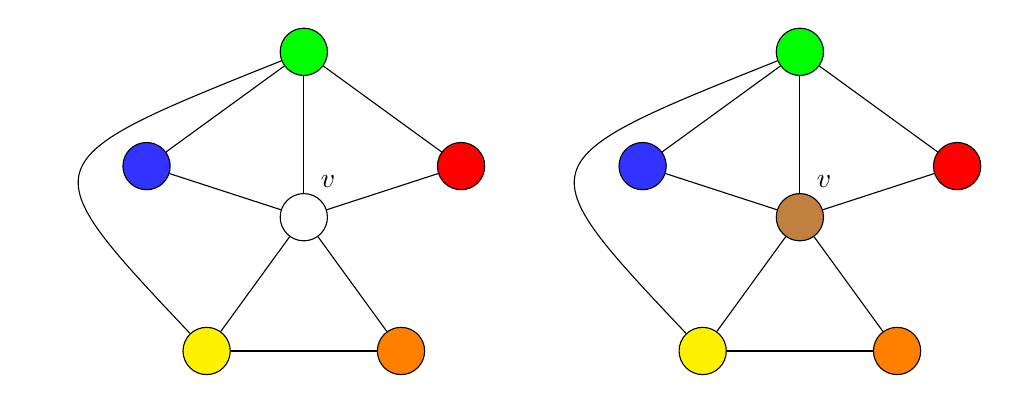
\begin{tikzpicture}[scale=.7,minimum size=6mm,inner sep=0pt]
\foreach \name/\color/\theta in
    {A/red/18,B/green/90,C/blue!80/162,D/yellow/234,E/orange/306}
  \node[circle,draw,fill=\color] (\name) at (\theta:3) {};
\node[circle,draw] (O) at (0,0) {};
\node[above right,yshift=4pt] at (O) {$v$};
\foreach \name in {A,B,C,D,E}
  \draw (O) -- (\name);
\foreach \i/\j in {A/B,B/C,D/E}
  \draw (\i) -- (\j);
\draw (B) .. controls (-5,1) .. (D);
\begin{scope}[xshift=9cm]
\foreach \name/\color/\theta in
    {A/red/18,B/green/90,C/blue!80/162,D/yellow/234,E/orange/306}
  \node[circle,draw,fill=\color] (\name) at (\theta:3) {};
\node[circle,draw,fill=brown] (O) at (0,0) {};
\node[above right,yshift=4pt] at (O) {$v$};
\foreach \name in {A,B,C,D,E}
  \draw (O) -- (\name);
\foreach \i/\j in {A/B,B/C,D/E}
  \draw (\i) -- (\j);
\draw (B) .. controls (-5,1) .. (D);
\end{scope}
\end{tikzpicture}
\end{center}

\selectlanguage{hebrew}


\section{משפט חמשת הצבעים}

\textbf{הגדרה:}
יהי
$G$
גרף מישורי מקושר צבוע. 
$G'$
הוא
\textbf{שרשרת}
אם ורק אם
$G'$
הוא תת-גרף מקסימלי של
$G$
הצבוע בשני צבעים.%
\footnote{%
השרשרת נקראת גם
\textbf{שרשרת \L{Kempe}}
כי היא הוגדרה על ידי
\L{Alfred Kempe}
בהוכחה השגויה שלו למשפט ארבעת הצבעים. ראו סעיף~%
\L{\ref{s.kempe}}.}

\begin{theorem}\label{thm.fivecolor}\mbox{}\\
כל גרף מישורי 
$G$
ניתן לצבוע בחמישה צבעים.
\end{theorem}

\textbf{הוכחה:}
באינדקציה על מספר הצמתים. נכונות המשפט ברורה עבור גרף מישורי עם חמישה צמתים או פחות.

יהי
$G$
גרף מישורי. לפי משפט
\L{~\ref{thm.degree5}}
קיים צומת
$v$
ממעלה חמש או פחות. מחק את הצומת
$v$
כדי לקבל את הגרף
$G'$.
לפי הנחת האינדוקציה, ניתן לצבוע את
$G'$
עם חמישה צבעים או פחות:


%\begin{figure}[tb]
\begin{center}

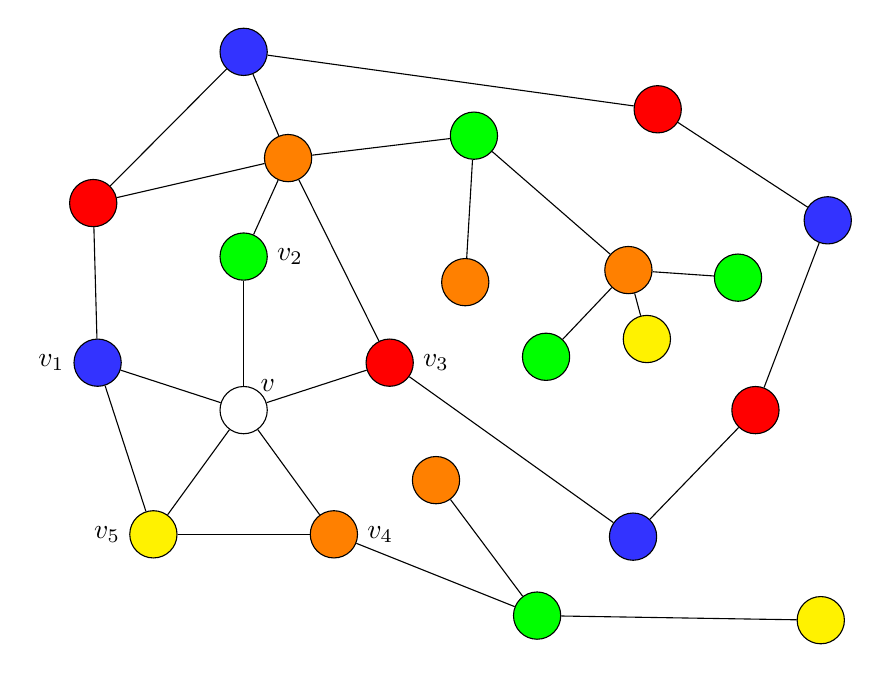
\begin{tikzpicture}[scale=.65,minimum size=6mm,inner sep=0pt]
\foreach \name/\color/\theta in
    {A/red/18,B/green/90,C/blue!80/162,D/yellow/234,E/orange/306}
  \node[circle,draw,fill=\color] (\name) at (\theta:3) {};
\node[circle,draw] (O) at (0,0) {};
\node[above right] at (O) {$v$};

\node[right,xshift=8pt] at (A) {$v_3$};
\node[right,xshift=8pt] at (B) {$v_2$};
\node[left,,xshift=-8pt] at (C) {$v_1$};
\node[left,,xshift=-8pt] at (D) {$v_5$};
\node[right,xshift=8pt] at (E) {$v_4$};

\foreach \name in {A,B,C,D,E}
  \draw (O) -- (\name);
  
\node[circle,draw,fill=red]  (X1) at (126:5) {};
\node[circle,draw,fill=blue!80] (X2) at (90:7)  {};
\node[circle,draw,fill=red]  (X3) at (36:10) {};
\node[circle,draw,fill=blue!80] (X4) at (18:12) {};
\node[circle,draw,fill=red]  (X5) at (0:10) {};
\node[circle,draw,fill=blue!80] (X6) at (-18:8) {};
\draw (C)  -- (X1);
\draw (X1) -- (X2);
\draw (X2) -- (X3);
\draw (X3) -- (X4);
\draw (X4) -- (X5);
\draw (X5) -- (X6);
\draw (X6) -- (A);

\node[circle,draw,fill=orange]  (Y1)  at (80:5) {};
\node[circle,draw,fill=green]   (Y2)  at (50:7)  {};
\node[circle,draw,fill=orange]  (Y3A) at (20:8) {};
\node[circle,draw,fill=orange]  (Y3B) at (30:5) {};
\node[circle,draw,fill=green]   (Y4A) at (10:6) {};
\node[circle,draw,fill=yellow]   (Y4B) at (10:8) {};
\node[circle,draw,fill=green]   (Y4C) at (15:10) {};
\node[circle,draw,fill=green]   (Y5)  at (-35:7) {};
\node[circle,draw,fill=yellow]  (Y6A) at (-20:12) {};
\node[circle,draw,fill=orange]  (Y6B) at (-20:4) {};
\draw (B)  -- (Y1);
\draw (Y1) -- (Y2);
\draw (Y2) -- (Y3A);
\draw (Y2) -- (Y3B);
\draw (Y3A) -- (Y4A);
\draw (Y3A) -- (Y4B);
\draw (Y3A) -- (Y4C);
\draw (E)  -- (Y5);
\draw (Y5) -- (Y6A);
\draw (Y5) -- (Y6B);
\draw (A) -- (Y1);
\draw (X2) -- (Y1);
\draw (X1) -- (Y1);
\draw (D) -- (E);
\draw (D) -- (C);
\end{tikzpicture}
\end{center}
%\caption{לצומת $v$ חמש שכנים לכל היותר}\label{f.five1}
%\end{figure}

ב-%
$G$,
אם המעלה של
$v$
היא פחות מחמש,
או אם
$v_1,\ldots,v_5$,
השכנים של
$v$,
צבועים עם ארבעה צבעים או פחות, ניתן לצבוע את
$v$
עם הצבע החמישי.
אחרת, הצמתים
$v_1,\ldots,v_5$
צבועים בצבעים שונים ב-%
$G'$
כמו באיור.

הצומת
$v_1$
צבוע בכחול והצומת 
$v_3$
צבוע באדום, ויש שרשרת הכחול-אדום המכילה אותם. על ידי הוספת הצומת 
$v$
והקשתות
$\overline{vv_1},\overline{vv_3}$
לשרשרת, נקבל מסלול סגור
$P$
)המסומן בקו כפול( שמחלק את המישור לשטח "פנימי" ולשטח "חיצוני" )אויר~%
\ref{f.five2}(.

\begin{figure}[tb]
\begin{center}

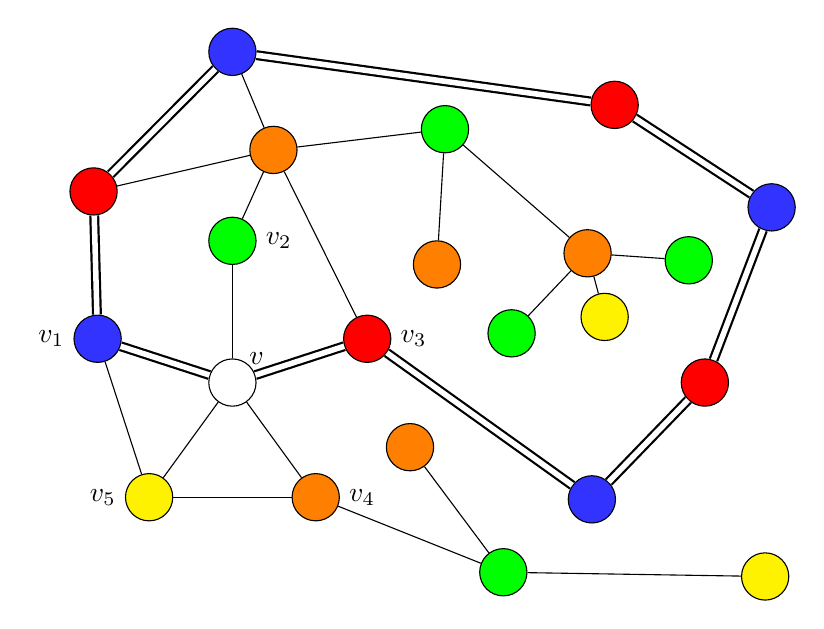
\begin{tikzpicture}[scale=.6,minimum size=6mm,inner sep=0pt]
\foreach \name/\color/\theta in
    {A/red/18,B/green/90,C/blue!80/162,D/yellow/234,E/orange/306}
  \node[circle,draw,fill=\color] (\name) at (\theta:3) {};
\node[circle,draw] (O) at (0,0) {};
\node[above right] at (O) {$v$};

\node[right,xshift=8pt] at (A) {$v_3$};
\node[right,xshift=8pt] at (B) {$v_2$};
\node[left,,xshift=-8pt] at (C) {$v_1$};
\node[left,,xshift=-8pt] at (D) {$v_5$};
\node[right,xshift=8pt] at (E) {$v_4$};

\foreach \name in {A,B,C,D,E}
  \draw (O) -- (\name);
  
\node[circle,draw,fill=red]  (X1) at (126:5) {};
\node[circle,draw,fill=blue!80] (X2) at (90:7)  {};
\node[circle,draw,fill=red]  (X3) at (36:10) {};
\node[circle,draw,fill=blue!80] (X4) at (18:12) {};
\node[circle,draw,fill=red]  (X5) at (0:10) {};
\node[circle,draw,fill=blue!80] (X6) at (-18:8) {};
\draw[thick,double distance=2pt] (C)  -- (X1);
\draw[thick,double distance=2pt] (X1) -- (X2);
\draw[thick,double distance=2pt] (X2) -- (X3);
\draw[thick,double distance=2pt] (X3) -- (X4);
\draw[thick,double distance=2pt] (X4) -- (X5);
\draw[thick,double distance=2pt] (X5) -- (X6);
\draw[thick,double distance=2pt] (X6) -- (A);
\draw[thick,double distance=2pt] (A) -- (O) -- (C);

\node[circle,draw,fill=orange]  (Y1)  at (80:5) {};
\node[circle,draw,fill=green]   (Y2)  at (50:7)  {};
\node[circle,draw,fill=orange]  (Y3A) at (20:8) {};
\node[circle,draw,fill=orange]  (Y3B) at (30:5) {};
\node[circle,draw,fill=green]   (Y4A) at (10:6) {};
\node[circle,draw,fill=yellow]   (Y4B) at (10:8) {};
\node[circle,draw,fill=green]   (Y4C) at (15:10) {};
\node[circle,draw,fill=green]   (Y5)  at (-35:7) {};
\node[circle,draw,fill=yellow]  (Y6A) at (-20:12) {};
\node[circle,draw,fill=orange]  (Y6B) at (-20:4) {};
\draw (B)  -- (Y1);
\draw (Y1) -- (Y2);
\draw (Y2) -- (Y3A);
\draw (Y2) -- (Y3B);
\draw (Y3A) -- (Y4A);
\draw (Y3A) -- (Y4B);
\draw (Y3A) -- (Y4C);
\draw (E)  -- (Y5);
\draw (Y5) -- (Y6A);
\draw (Y5) -- (Y6B);
\draw (A) -- (Y1);
\draw (X2) -- (Y1);
\draw (X1) -- (Y1);
\draw (D) -- (E);
\draw (D) -- (C);
\end{tikzpicture}
\end{center}
\selectlanguage{hebrew}
\caption{מסלול מחלק את המישור לחלק פנימי ולחלק חיצוני}\label{f.five2}
\end{figure}
כעת נתבונן בצומת
$v_2$
הצבוע ירוק ובצומת
$v_4$
הצבוע כתום. הצמתים הללו 
\textbf{אינם}
יכולים להיות בשרשרת ירוק-כתום אחת, כי 
$v_2$
נמצא 
\textbf{בתוך}
$P$
ו-%
$v_4$
נמצא
\textbf{מחוץ}
ל-%
$P$,
ולכן כל מסלול המחבר אותם חייב לחתוך את
$P$,
הסותר את ההנחה שהגרף מישורי.%
\footnote{\R{טענה זו נובעת מה}-%
\L{\emph{Jordan curve theorem}},
\R{שהוא ברור באופן אינטואיטיבי, אבל קשה מאוד להוכיח}.}
באיור~%
\ref{f.five3}
אפשר לראות שתי שרשראות ירוק-כתום המכילות את
$v_2$
ו-%
$v_4$
שאינן מחוברות )מסומנות בקו מקווקוו כפול(.
\begin{figure}[tb]
\begin{center}

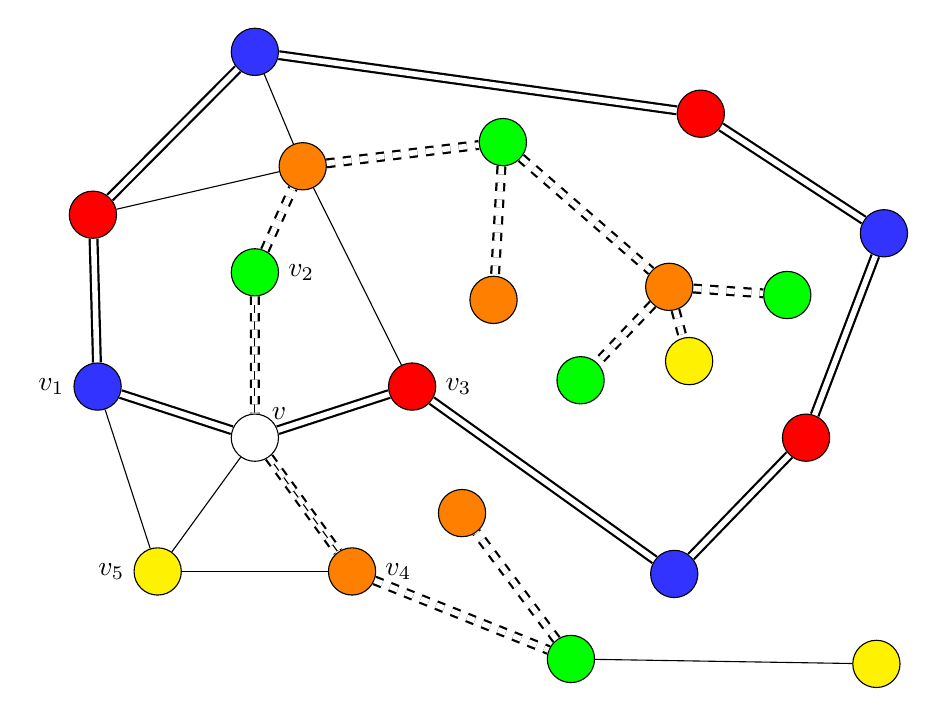
\begin{tikzpicture}[scale=.7,minimum size=6mm,inner sep=0pt]
\foreach \name/\color/\theta in
    {A/red/18,B/green/90,C/blue!80/162,D/yellow/234,E/orange/306}
  \node[circle,draw,fill=\color] (\name) at (\theta:3) {};
\node[circle,draw] (O) at (0,0) {};
\node[above right] at (O) {$v$};

\node[right,xshift=8pt] at (A) {$v_3$};
\node[right,xshift=8pt] at (B) {$v_2$};
\node[left,,xshift=-8pt] at (C) {$v_1$};
\node[left,,xshift=-8pt] at (D) {$v_5$};
\node[right,xshift=8pt] at (E) {$v_4$};

\foreach \name in {A,B,C,D,E}
  \draw (O) -- (\name);
  
\node[circle,draw,fill=red]  (X1) at (126:5) {};
\node[circle,draw,fill=blue!80] (X2) at (90:7)  {};
\node[circle,draw,fill=red]  (X3) at (36:10) {};
\node[circle,draw,fill=blue!80] (X4) at (18:12) {};
\node[circle,draw,fill=red]  (X5) at (0:10) {};
\node[circle,draw,fill=blue!80] (X6) at (-18:8) {};

\draw[thick,double distance=2pt] (C)  -- (X1);
\draw[thick,double distance=2pt] (X1) -- (X2);
\draw[thick,double distance=2pt] (X2) -- (X3);
\draw[thick,double distance=2pt] (X3) -- (X4);
\draw[thick,double distance=2pt] (X4) -- (X5);
\draw[thick,double distance=2pt] (X5) -- (X6);
\draw[thick,double distance=2pt] (X6) -- (A);
\draw[thick,double distance=2pt] (A) -- (O) -- (C);

\node[circle,draw,fill=orange]  (Y1)  at (80:5) {};
\node[circle,draw,fill=green]   (Y2)  at (50:7)  {};
\node[circle,draw,fill=orange]  (Y3A) at (20:8) {};
\node[circle,draw,fill=orange]  (Y3B) at (30:5) {};
\node[circle,draw,fill=green]   (Y4A) at (10:6) {};
\node[circle,draw,fill=yellow]   (Y4B) at (10:8) {};
\node[circle,draw,fill=green]   (Y4C) at (15:10) {};
\node[circle,draw,fill=green]   (Y5)  at (-35:7) {};
\node[circle,draw,fill=yellow]  (Y6A) at (-20:12) {};
\node[circle,draw,fill=orange]  (Y6B) at (-20:4) {};
\draw[thick,dashed,double distance=2pt] (B)  -- (O) -- (E);
\draw[thick,dashed,double distance=2pt] (B)  -- (Y1);
\draw[thick,dashed,double distance=2pt] (Y1) -- (Y2);
\draw[thick,dashed,double distance=2pt] (Y2) -- (Y3A);
\draw[thick,dashed,double distance=2pt] (Y2) -- (Y3B);
\draw[thick,dashed,double distance=2pt] (Y3A) -- (Y4A);
\draw[thick,dashed,double distance=2pt] (Y3A) -- (Y4B);
\draw[thick,dashed,double distance=2pt] (Y3A) -- (Y4C);
\draw[thick,dashed,double distance=2pt] (E)  -- (Y5);
\draw[thick,dashed,double distance=2pt] (Y5) -- (Y6B);
\draw (Y5) -- (Y6A);
\draw (A) -- (Y1);
\draw (X2) -- (Y1);
\draw (X1) -- (Y1);
\draw (D) -- (E);
\draw (D) -- (C);
\end{tikzpicture}
\end{center}
\selectlanguage{hebrew}
\caption{שרשראות לא מחוברות}\label{f.five3}
\end{figure}

נחליף ביניהם את שני ההצבעים בשרשרת המכילה את
$v_2$
)איור~%
\ref{f.five4}(.
עדיין ניתן לצבוע את
$G'$
עם חמישה צבעים.
$v_2$
ו-%
$v_4$
שניהם צבועים בכתום, וניתן לצבוע את
$v$
בירוק כדי לקבל צביעה של
$G$
עם חמישה צבעים.
\qed

\begin{figure}[tb]
\begin{center}

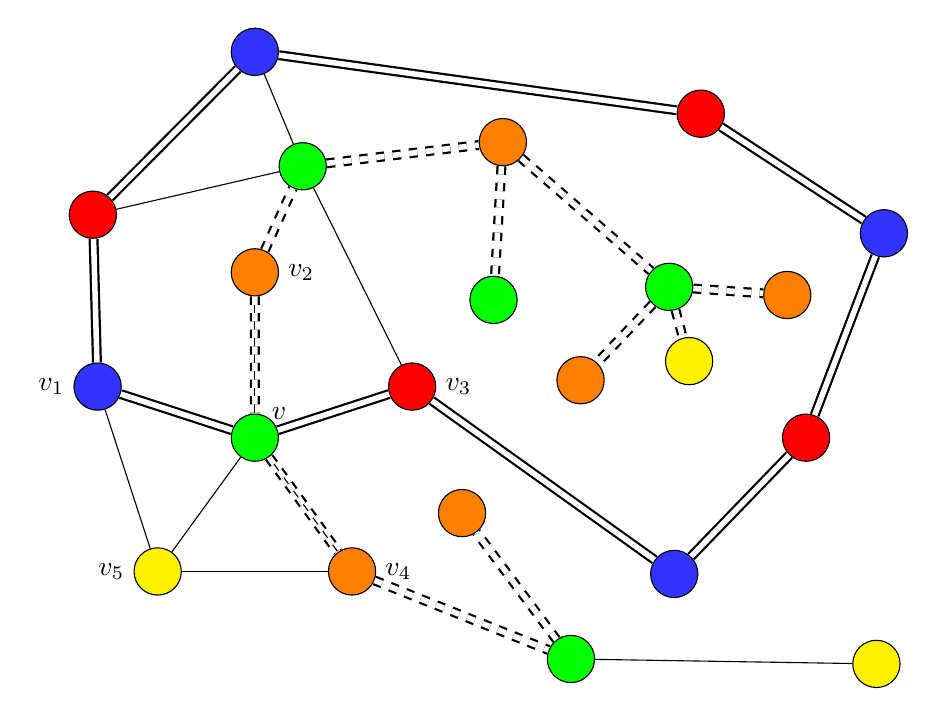
\begin{tikzpicture}[scale=.7,minimum size=6mm,inner sep=0pt]
\foreach \name/\color/\theta in
    {A/red/18,B/orange/90,C/blue!80/162,D/yellow/234,E/orange/306}
  \node[circle,draw,fill=\color] (\name) at (\theta:3) {};
\node[circle,draw,fill=green] (O) at (0,0) {};
\node[above right] at (O) {$v$};

\node[right,xshift=8pt] at (A) {$v_3$};
\node[right,xshift=8pt] at (B) {$v_2$};
\node[left,,xshift=-8pt] at (C) {$v_1$};
\node[left,,xshift=-8pt] at (D) {$v_5$};
\node[right,xshift=8pt] at (E) {$v_4$};

\foreach \name in {A,B,C,D,E}
  \draw (O) -- (\name);
  
\node[circle,draw,fill=red]  (X1) at (126:5) {};
\node[circle,draw,fill=blue!80] (X2) at (90:7)  {};
\node[circle,draw,fill=red]  (X3) at (36:10) {};
\node[circle,draw,fill=blue!80] (X4) at (18:12) {};
\node[circle,draw,fill=red]  (X5) at (0:10) {};
\node[circle,draw,fill=blue!80] (X6) at (-18:8) {};

\draw[thick,double distance=2pt] (C)  -- (X1);
\draw[thick,double distance=2pt] (X1) -- (X2);
\draw[thick,double distance=2pt] (X2) -- (X3);
\draw[thick,double distance=2pt] (X3) -- (X4);
\draw[thick,double distance=2pt] (X4) -- (X5);
\draw[thick,double distance=2pt] (X5) -- (X6);
\draw[thick,double distance=2pt] (X6) -- (A);
\draw[thick,double distance=2pt] (A) -- (O) -- (C);

\node[circle,draw,fill=green]  (Y1)  at (80:5) {};
\node[circle,draw,fill=orange]   (Y2)  at (50:7)  {};
\node[circle,draw,fill=green]  (Y3A) at (20:8) {};
\node[circle,draw,fill=green]  (Y3B) at (30:5) {};
\node[circle,draw,fill=orange]   (Y4A) at (10:6) {};
\node[circle,draw,fill=yellow]   (Y4B) at (10:8) {};
\node[circle,draw,fill=orange]   (Y4C) at (15:10) {};
\node[circle,draw,fill=green]   (Y5)  at (-35:7) {};
\node[circle,draw,fill=yellow]  (Y6A) at (-20:12) {};
\node[circle,draw,fill=orange]  (Y6B) at (-20:4) {};

\draw[thick,dashed,double distance=2pt] (B)  -- (O) -- (E);
\draw[thick,dashed,double distance=2pt] (B)  -- (Y1);
\draw[thick,dashed,double distance=2pt] (Y1) -- (Y2);
\draw[thick,dashed,double distance=2pt] (Y2) -- (Y3A);
\draw[thick,dashed,double distance=2pt] (Y2) -- (Y3B);
\draw[thick,dashed,double distance=2pt] (Y3A) -- (Y4A);
\draw[thick,dashed,double distance=2pt] (Y3A) -- (Y4B);
\draw[thick,dashed,double distance=2pt] (Y3A) -- (Y4C);
\draw[thick,dashed,double distance=2pt] (E)  -- (Y5);
\draw[thick,dashed,double distance=2pt] (Y5) -- (Y6B);

\draw (Y5) -- (Y6A);
\draw (A) -- (Y1);
\draw (X2) -- (Y1);
\draw (X1) -- (Y1);
\draw (D) -- (E);
\draw (D) -- (C);
\end{tikzpicture}
\end{center}
\selectlanguage{hebrew}
\caption{החלפת צבעים בשרשרת אחת}\label{f.five4}
\end{figure}

%%%%%%%%%%%%%%%%%%%%%%%%%%%%%%%%%%%%%%%%%%%%%%%%%%%%%%%%%%%
%%%%%%%%%%%%%%%%%%%%%%%%%%%%%%%%%%%%%%%%%%%%%%%%%%%%%%%%%%%

\section{ההוכחה השגויה של
\L{Kempe}
לבעיית ארבע הצבעים}
\label{s.kempe}

משפט ארבעת הצבעים הוצג כהשערה ב-%
$1852$.
ב-%
$1879$
\L{Alfred B. Kempe}
פרסם הוכחה, אבל ב-%
$1890$,
\L{Percy J. Heawood}
מצא בה שגיאה. העבודה של
\L{Kempe}
חשובה כי: 
$(1)$
ההוכחה נכונה עבור חמישה צבעים, ו-%
$(2)$
בהוכחה שלו הוא המציא את הרעיונות הבסיסיים ששימשו את
\L{Appel}
ו-%
\L{Haken}
בהוכחה הנכונה שלהם שפורסמה ב-%
$1976$.

\textbf{"הוכחה":}
רוב ההוכחה זהה להוכחה של משפט חמשת הצבעים. המקרה החדש הוא צומת 
$v$
עם חמישה שכנים שלפי ההנחה האינדוקטיבית ניתן לצבוע אותם
\textbf{בארבעה}
צבעים לאחר מחיקת הצומת
$v$.

בגרף השמאלי של איור %
\ref{f.kempe1}
קיימים שני צמתים
$v_2,v_5$
הצבועים בכחול. נתבונן עכשיו בשרשרת הכחול-ירוק המכילה את 
$v_2$
ובשרשרת הכחול-צהוב המכילה את
$v_5$.
השרשרת הכחול-ירוק נמצאת מתוך המסלול הסגור המוגדר על ידי השרשרת האדום-צהוב שמכילה את
$v_1,v_3$
)מסומן בקו כפול(,
והשרשרת הכחול-צהוב נמצאת בתוך המסלול הסגור המוגדר על ידי השרשרת האדום-ירוק המכילה את
$v_1,v_4$
(מסומן בקו כפול מקווקוו(.

נחליף את הצבעים בשרשרת הכחול-ירוק ובשרשרת הכחול-צהוב )איור ימני(. השכנים של
$v$
צבועים בשלושה צבעים )אדום, ירוק צהוב( וניתן לצבוע את
$v$
בכחול.
\qed
\begin{figure}
\begin{center}

\begin{tikzpicture}[scale=.6,minimum size=6mm,inner sep=0pt]

% Draw center node and adjacent nodes
\foreach \name/\color/\theta in
    {A/yellow/18,B/blue!80/90,C/red/162,D/blue!80/234,E/green/306}
  \node[circle,draw,fill=\color] (\name) at (\theta:3) {};
\node[circle,draw] (O) at (0,0) {};
\node[above right]     at (O) {$v$};

\node[right,xshift=10pt] at (A) {$v_3$};
\node[left,xshift=-8pt]  at (B) {$v_2$};
\node[left,xshift=-8pt]  at (C) {$v_1$};
\node[left,xshift=-8pt]  at (D) {$v_5$};
\node[right,xshift=8pt]  at (E) {$v_4$};

% Draw red-yellow path
\node[circle,draw,fill=yellow]  (X1) at (126:5) {};
\node[circle,draw,fill=red] (X2) at (45:8)  {};

\draw[thick,double distance=2pt] 
  (C) -- (X1) -- (X2) -- (A) -- (O);
\draw[thick,double distance=6pt] (O) -- (C);

% Draw blue-green nodes within red-yellow path
\node[circle,draw,fill=green] (Y1)  at (50:5) {};

% Draw red-green path
\node[circle,draw,fill=green] (Z1)  at (-160:5) {};
\node[circle,draw,fill=red]   (Z2)  at (-80:6)  {};

%\draw[thick,dashed,double distance=6pt] (O) -- (C);
\draw[thick,dashed,double distance=2pt] 
  (O) -- (C) -- (Z1) -- (Z2) -- (E) -- (O);

% Draw blue-yellow nodes within red-green path
\node[circle,draw,fill=yellow]   (U1)  at (-90:4)  {};

% Connect adjacent nodes not in paths
\draw (X1) -- (B) -- (Y1) -- (A) -- (B) -- 
      (C) -- (D) -- (E) -- (A);
\draw (Z2) -- (U1) -- (D) -- (O) -- (B);

%\end{tikzpicture}
%\end{center}

\begin{scope}[xshift=12cm]
%\begin{center}
%\begin{tikzpicture}[scale=.6,minimum size=6mm,inner sep=0pt]

% Draw center node and adjacent nodes
\foreach \name/\color/\theta in
    {A/yellow/18,B/green/90,C/red/162,D/yellow/234,E/green/306}
  \node[circle,draw,fill=\color] (\name) at (\theta:3) {};
\node[circle,draw,fill=blue!80] (O) at (0,0) {};
\node[above right]     at (O) {$v$};

\node[right,xshift=10pt] at (A) {$v_3$};
\node[left,xshift=-8pt]  at (B) {$v_2$};
\node[left,xshift=-8pt]  at (C) {$v_1$};
\node[left,xshift=-8pt]  at (D) {$v_5$};
\node[right,xshift=8pt]  at (E) {$v_4$};

% Draw red-yellow path
\node[circle,draw,fill=yellow]  (X1) at (126:5) {};
\node[circle,draw,fill=red] (X2) at (45:8)  {};

\draw[thick,double distance=2pt] 
  (C) -- (X1) -- (X2) -- (A) -- (O);
\draw[thick,double distance=6pt] (O) -- (C);

% Draw blue-green nodes within red-yellow path
\node[circle,draw,fill=blue!80] (Y1)  at (50:5) {};

% Draw red-green path
\node[circle,draw,fill=green] (Z1)  at (-160:5) {};
\node[circle,draw,fill=red]   (Z2)  at (-80:6)  {};

\draw[thick,dashed,double distance=2pt] 
  (O) -- (C) -- (Z1) -- (Z2) -- (E) -- (O);

% Draw blue-yellow nodes within red-green path
\node[circle,draw,fill=blue!80]   (U1)  at (-90:4)  {};

% Connect adjacent nodes not in paths
\draw (X1) -- (B) -- (Y1) -- (A) -- (B) -- 
      (C) -- (D) -- (E) -- (A);
\draw (Z2) -- (U1) -- (D) -- (O) -- (B);
\end{scope}
\end{tikzpicture}
\end{center}
\selectlanguage{hebrew}
\caption{ההוכחה המוטעת של Kempe}\label{f.kempe1}
\end{figure}

\L{Heawood}
שם לב שלמסלולים הסגורים, המוגדרים על ידי השרשראות האדום-צהוב והאדום-ירוק, ייתכן שיש צמתים אדומים משותפים )%
$v_1$
והצומת האדום מתחת ל-%
$v_4$
בגרף השמאלי של איור~%
\ref{f.kempe2}(.
כאשר מחליפים צבעים בשרשראות הכחול-ירוק והכחול-צהוב, יש אפשרות שיהיו צמתים צבועים בכחול הקשורים בקשת )איור ימני(, כך שהצביעה כבר לא חוקית.
\begin{figure}[tb]
\begin{center}

\begin{tikzpicture}[scale=.6,minimum size=6mm,inner sep=0pt]

% Draw center node and adjacent nodes
\foreach \name/\color/\theta in
    {A/yellow/18,B/blue!80/90,C/red/162,D/blue!80/234,E/green/306}
  \node[circle,draw,fill=\color] (\name) at (\theta:3) {};
\node[circle,draw] (O) at (0,0) {};
\node[above right]     at (O) {$v$};

\node[right,xshift=10pt] at (A) {$v_3$};
\node[right,xshift=8pt]  at (B) {$v_2$};
\node[above right,xshift=8pt]  at (C) {$v_1$};
\node[below right,yshift=-8pt] at (D) {$v_5$};
\node[right,xshift=8pt]  at (E) {$v_4$};

% Draw red-yellow path
\node[circle,draw,fill=yellow] (X1) at (-170:5) {};
\node[circle,draw,fill=red]    (X2) at (-80:7)  {};

\draw[thick,double distance=2pt] (A) -- (O);
\draw[thick,double distance=6pt] (O) -- (C);
\draw[thick,double distance=2pt] (C) --(X1) -- (X2);
\draw[thick,double distance=2pt,bend right=40] (X2) to (A);

% Draw red-green path
\node[circle,draw,fill=green] (Y1) at (100:6)  {};

\draw[dashed,thick,double distance=2pt] (O) -- (C) -- (Y1);
\draw[dashed,thick,double distance=2pt] 
  (Y1) .. controls (40:10) and (-50:9) .. (X2);
\draw[dashed,thick,double distance=2pt] (X2) -- (E) -- (O);

% Draw adjacent nodes
\draw (X1) -- (D) -- (O) -- (B) -- (Y1) -- (X1);

%\end{tikzpicture}
%\end{center}

\begin{scope}[xshift=12cm]
%\begin{center}
%\begin{tikzpicture}[scale=.6,minimum size=6mm,inner sep=0pt]

% Draw center node and adjacent nodes
\foreach \name/\color/\theta in
    {A/yellow/18,B/green/90,C/red/162,D/yellow/234,E/green/306}
  \node[circle,draw,fill=\color] (\name) at (\theta:3) {};
\node[circle,draw,fill=blue!80] (O) at (0,0) {};
\node[above right]     at (O) {$v$};

\node[right,xshift=10pt] at (A) {$v_3$};
\node[right,xshift=8pt]  at (B) {$v_2$};
\node[above right,xshift=8pt]  at (C) {$v_1$};
\node[below right,yshift=-8pt] at (D) {$v_5$};
\node[right,xshift=8pt]  at (E) {$v_4$};


% Draw red-yellow path
\node[circle,draw,fill=blue!80] (X1) at (-170:5) {};
\node[circle,draw,fill=red]  (X2) at (-80:7)  {};

\draw[thick,double distance=2pt] (A) -- (O);
\draw[thick,double distance=6pt] (O) -- (C);
\draw[thick,double distance=2pt] (C) --(X1) -- (X2);
\draw[thick,double distance=2pt,bend right=40] (X2) to (A);

% Draw red-green path
\node[circle,draw,fill=blue!80] (Y1) at (100:6)  {};

\draw[dashed,thick,double distance=2pt] (O) -- (C) -- (Y1);
\draw[dashed,thick,double distance=2pt] 
  (Y1) .. controls (40:10) and (-50:9) .. (X2);
\draw[dashed,thick,double distance=2pt] (X2) -- (E) -- (O);

% Draw adjacent nodes
\draw (X1) -- (D) -- (O) -- (B) -- (Y1) -- (X1);
\end{scope}
\end{tikzpicture}
\end{center}
\selectlanguage{hebrew}
\caption{השגיאה בהוכחה ש-Heawood מצא}\label{f.kempe2}
\end{figure}


\selectlanguage{hebrew}


\subsection*{מקורות}
על משפט ארבעת הצבעים ראו 
\L{\cite{thomas}, \cite{wiki:four}}.
ההוכחה של משפט חמשת הצבעים לקוחה מ-%
\L{\cite{thebook}, \cite{wiki:five}}.
\L{\cite{eppstein}}
מביא הוכחות רבות לנוסחת
\L{Euler}.
השגיאה בהוכחה של 
\L{Kempe}
מתוארת ב-%
\L{\cite{sipka}}.
